Control signals can be communicated separately from the USB interface using the serial port on the RTSC.  PC serial ports conform to the RS232 standard which uses signaling voltages that are incompatible with the 3.3VTTL/CMOS logic of the FPGA~\cite{StrangioRS232}.  The ST232 level shifting IC converts logic LOW and HIGH of LVTTL/CMOS voltages to RS232 compatible voltages without the need for higher voltage supplies~\cite{ST232ds}.  Table~\ref{tab:RS232TTL} shows the logic voltage levels compatible with the Xilinx\textsuperscript{\textregistered} XC3S500E FPGA IO pins configured for LVTTL and logic voltages compatible with the RS232 standard~\cite{Spartan3eDS,StrangioRS232}.

\renewcommand{\arraystretch}{1.3}
\begin{table}[h]
\centering 
  \begin{tabular}{| l | c | c | c | c |}
    \hline
    Logic & LOW$_{\mathrm{min}}$ & LOW$_{\mathrm{max}}$ & HIGH$_{\mathrm{min}}$ & HIGH$_{\mathrm{max}}$ \\
	\hline
    LVTTL & $-0.5\unit{V}$ & $+0.8\unit{V}$ & $+2.0\unit{V}$ & $+3.8\unit{V}$ \\
	\hline
    RS232 & $+3.0\unit{V}$ & $+25.0\unit{V}$ & $-25.0\unit{V}$  & $-3.0\unit{V}$ \\
    \hline
  \end{tabular}
  \caption{FPGA and RS232 logic voltage level comparison\label{tab:RS232TTL} }

\end{table}
\renewcommand{\arraystretch}{1.0}

RS232 communication is asynchronous and full duplex with separate receive (often labeled as RX or R) and transmit (often labeled as TX or T) data lines and without a dedicated clock signal.  The signals other than RX and TX are not necessary for simple communication between one host and peripheral~\cite{StrangioRS232}.

As shown in Figure~\ref{fig:RS232}, the ST232 level shifting IC is between the FPGA's GPIO pins being used for RX and TX signals that can be connected to a PC via the standard pinout D-Subminiature 9 pin (DB9) connector.  The ST232 is capable of passing two separate RS232 communication busses (R1/T1 IN/OUT and R2/T2 IN/OUT), but only one set is used by the FPGA.

\begin{figure}[H]
	\centering 
		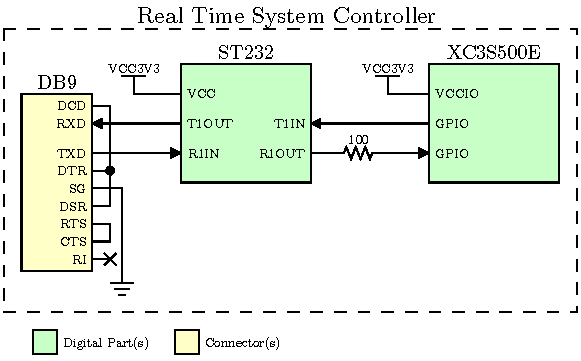
\includegraphics{./figures/RS232} 
	\caption{RS232 level shifter that allows a PC serial port to communicate with the FPGA~\cite{DigilentNexys2rm,DigilentNexys2sch}\label{fig:RS232}}
\end{figure}

For a future design, an alternative to provide PC communication is to use an TTL-232RG cable from FTDI that connects to a USB port and provides a virtual serial port to the PC while providing a TTL serial UART compatible interface to connect to the FPGA, directly~\cite{FTDIUSBSerial}.

%A series resistor is placed between the FPGA's RX GPIO pin and the R1OUT of the ST232  to limit current into an unpowered Nexys2 if a PC or other device is connected to the DB9.


